\clearpage
\pagenumbering{arabic}
\setcounter{page}{1}

\phantomsection
\label{ch:intro}
\chapter{Introduction}

This chapter presents about what is OCR? why it is needed, and
what are the challenges in OCR. It also presents the problem 
for OCR on Khmer script (non-latin based), and OCR on multilingual
language such as Khmer and English. We will talk about the scope
of this research because it'll help us to keep 
our research scope ensures clarity, direction, and feasibility 
throughout the study.

\section{Background to the Study}
\label{sec:background}

Optical Character Recognition (OCR) has changed how we turn printed text into digital formats. Thanks to AI advances, OCR systems now use deep learning to detect and classify characters from images. This technology powers digital libraries, search systems, and language processing tools.

OCR works great for major languages like English, Chinese, and Japanese. These languages have tons of training data and well-studied text structures. But OCR for smaller languages like Khmer? That's a different story.

Cambodia needs OCR technology more than ever. Over the past 20 years, the country has gone digital fast. People want to digitize Khmer documents for education, research, and everyday use. But here's the problem: Khmer script is incredibly complex.

Khmer writing goes back to the 7th century. It's not like English where letters sit in a row. Khmer characters stack on top of each other. They have subscripts, diacritics, and vowel markers that can appear above, below, or around the main character. Miss one tiny mark and you change the whole meaning of a word.

\begin{table}[H]
    \caption{Why Khmer OCR is Desperately Needed}
    \vspace{10pt}
    \phantomsection
    \label{sec:textbook}
    \resizebox{\textwidth}{!}{
    \begin{tabular}{|l|l|l|}
    \hline
    Sector & Current Problem & Impact \\
    \hline
    Education & Physical textbooks only & Students can't search or edit content \\
    Libraries & Books rotting on shelves & Knowledge becomes inaccessible \\
    Government & Paper records everywhere & Slow bureaucracy, hard to find documents \\
    Healthcare & Handwritten patient files & Doctors waste time, medical errors increase \\
    Business & Manual data entry & Companies lose money on inefficiency \\
    Culture & Ancient texts deteriorating & We're losing our heritage \\
    \hline
    \end{tabular}
    }
\end{table}

Look at education. Most school textbooks exist only on paper. The original digital files? Gone. Lost. This creates real problems for students who need accessible learning materials.

But it's bigger than just schools. Ancient palm leaf manuscripts are crumbling. Government documents pile up in storage rooms. Hospitals still use paper files that doctors can't read properly. Businesses waste hours typing data that OCR could handle in minutes.

And here's what's really frustrating: while Google can read English text perfectly, it struggles with basic Khmer sentences. The technology gap is huge.

The thing is, Khmer OCR isn't just a nice to have anymore. It's essential for Cambodia's digital future. The country needs this technology to preserve its culture, modernize its institutions, and give its people better access to information.

That's exactly why this research matters. We're not just building another OCR system. We're creating technology that could unlock thousands of years of Khmer knowledge and make it searchable, editable, and accessible to everyone.


\section{Problem Statement}
\label{sec:problem}

To develop OCR for English is really hard, but the way much more harder than you think is 
OCR on mixing languages such as English and Khmer. Most OCR systems work great with English because English is simple. Letters sit 
in a line. You read left to right, and Done.

For Khmer, that's a completely different beast. Characters stack on top of each other. 
They have tiny marks above and below that change the meaning. Miss one little dot 
and you've got the wrong word entirely.

\begin{figure}[H]
    \centering
    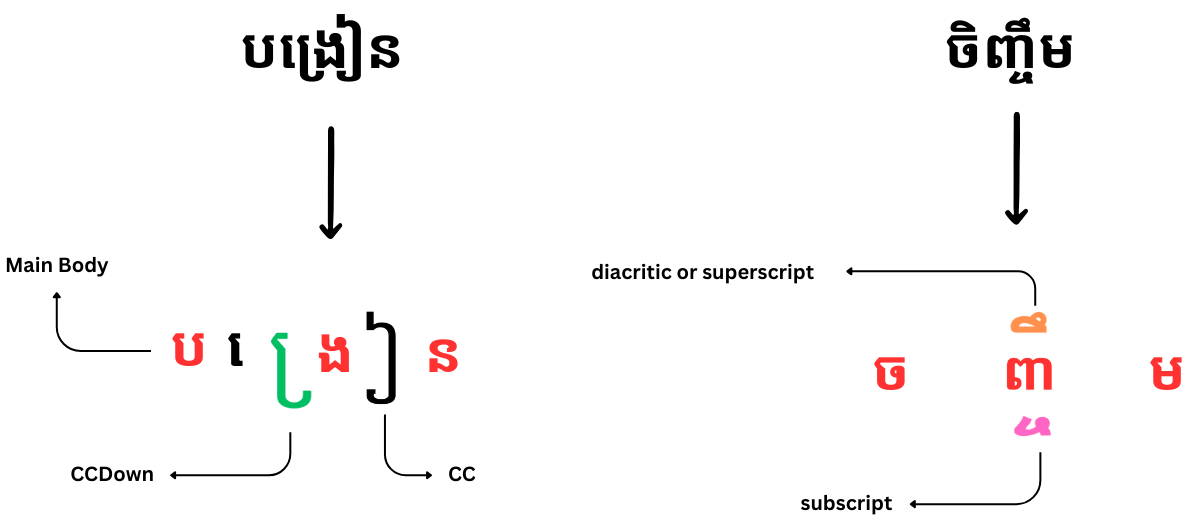
\includegraphics[width=\textwidth]{figures/example_of_text_format.png}
    \caption{Example of Khmer text format showing the complexity of character combinations and diacritics}
    \label{fig:text_format}
\end{figure}

Here's what makes Khmer OCR so different. First, there are no clear word breaks. 
In English, they use spaces between words (it's easy for AI to detect word level). 
Khmer writers use spaces sometimes, sometimes they don't, as you can see in figure
\ref{fig:sequential_text}, so it's really inconsistencies wirting system. This 
makes it impossible to know where one word ends and another begins.

\begin{figure}[H]
    \centering
    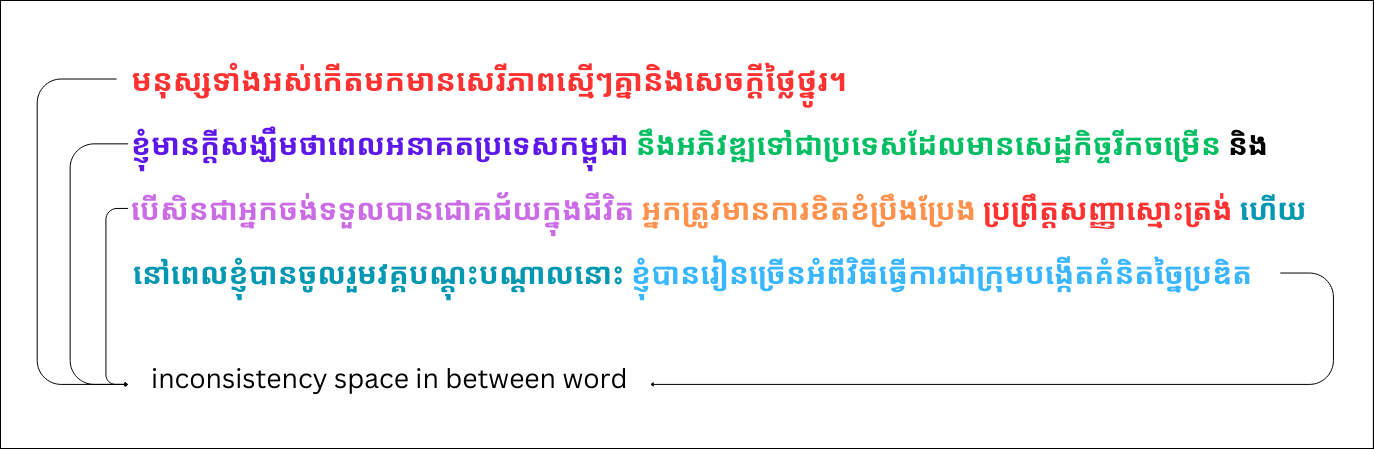
\includegraphics[width=\textwidth]{figures/example_of_long_text.png}
    \caption{Example of sequential Khmer text showing how characters combine to form syllables and words}
    \label{fig:sequential_text}
\end{figure}

A growing challenge in modern Cambodia is the increasing prevalence of mixed-language 
documents that combine Khmer and English text. As English education and international 
business have expanded over the past two decades, it's become common to see documents, 
signs, textbooks, and digital content that seamlessly blend both languages within the 
same sentence or paragraph.

\begin{figure}[H]
    \centering
    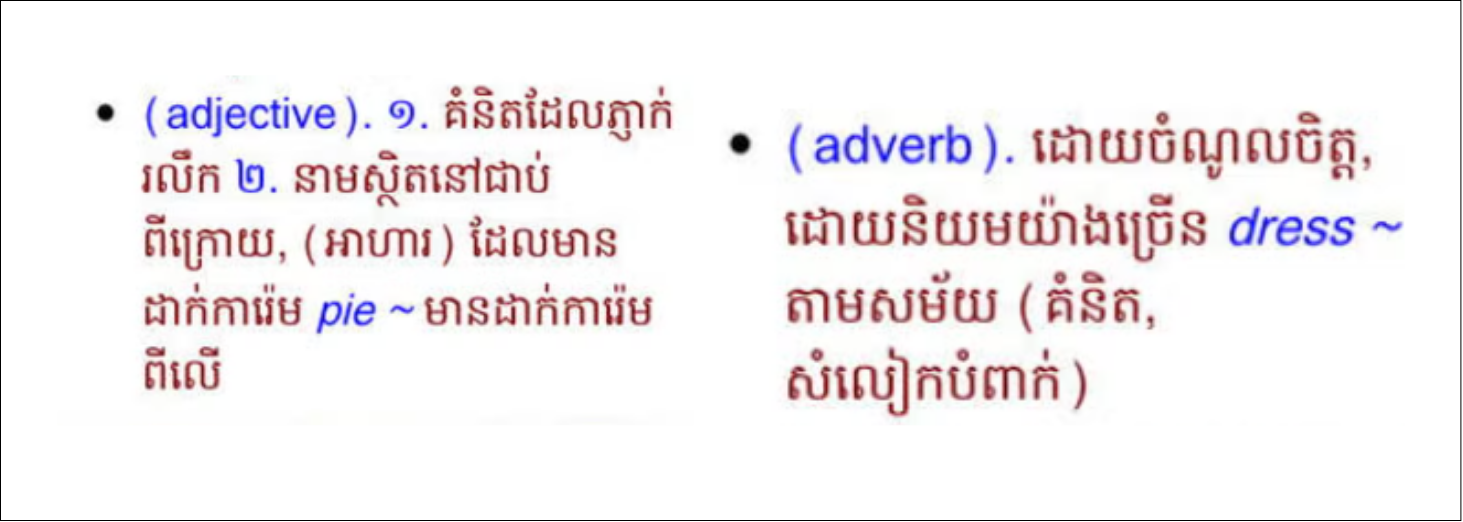
\includegraphics[width=\textwidth]{figures/mix_language_khmer_and_english.png}
    \caption{Example of mixed Khmer-English text showing how both languages appear together in modern Cambodian documents}
    \label{fig:mix_language}
\end{figure}

This mixed-language phenomenon creates several specific problems for OCR systems:
\begin{itemize}
    \item \textbf{Script switching confusion:} OCR models must quickly adapt between completely different writing systems within the same text line
    \item \textbf{Different text layouts:} English flows horizontally while Khmer has vertical stacking, creating complex spatial relationships
    \item \textbf{Font inconsistencies:} The same document often uses different fonts for Khmer and English portions, confusing recognition model
\end{itemize}

Most existing Khmer OCR systems are designed for single-language scenarios 
and perform poorly when encountering this mixed-language reality 
that's everywhere in Cambodia today. Then there's the data problem. To develop high 
accuracy OCR model needs tons of millions annotated images. English has millions 
of labeled images already, How about Khmer lanugage? 
Finding sufficient training data presents a significant challenge. 
While English has millions of labeled training samples, Khmer language 
resources are extremely limited, with only a few thousand quality annotated 
samples available. The situation becomes even more challenging when seeking 
properly labeled mixed-language datasets that combine Khmer and English text. Without enough 
training data, OCR model stays dumb. It can't learn the 
patterns to recognize text accurately.

\begin{figure}[H]
    \centering
    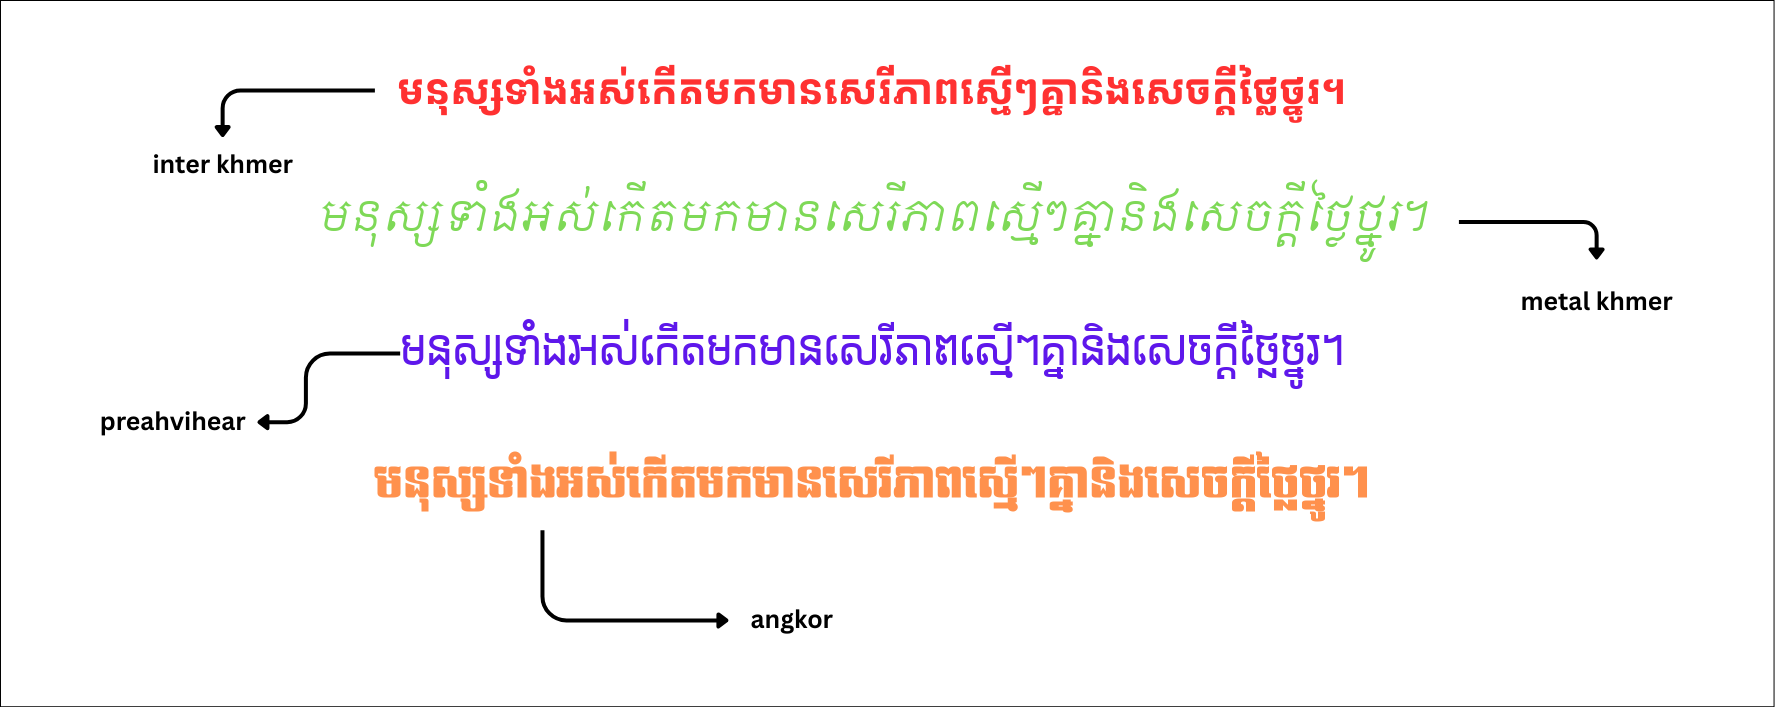
\includegraphics[width=\textwidth]{figures/varianty_of_font.png}
    \caption{Examples of the same Khmer text rendered in different fonts, demonstrating the significant visual variations that OCR systems must handle}
    \label{fig:font_variants}
\end{figure}

And let's talk about fonts. English has maybe around 15 to 25 common fonts that most people use,
based on reported study use case, from website such as rigorousthemes.com, lifehack.org, and indeed.com. 
Khmer has many different fonts that look very unique from each other, some are thick and bold, others are 
thin and delicate, some have fancy decorations. To train model on one font and 
it fails completely on another.

Look at Figure \ref{fig:font_variants}. Same text, different fonts. To a human, 
it's obviously the same sentence, to a computer, it might be different look.

\begin{figure}[H]
    \centering
    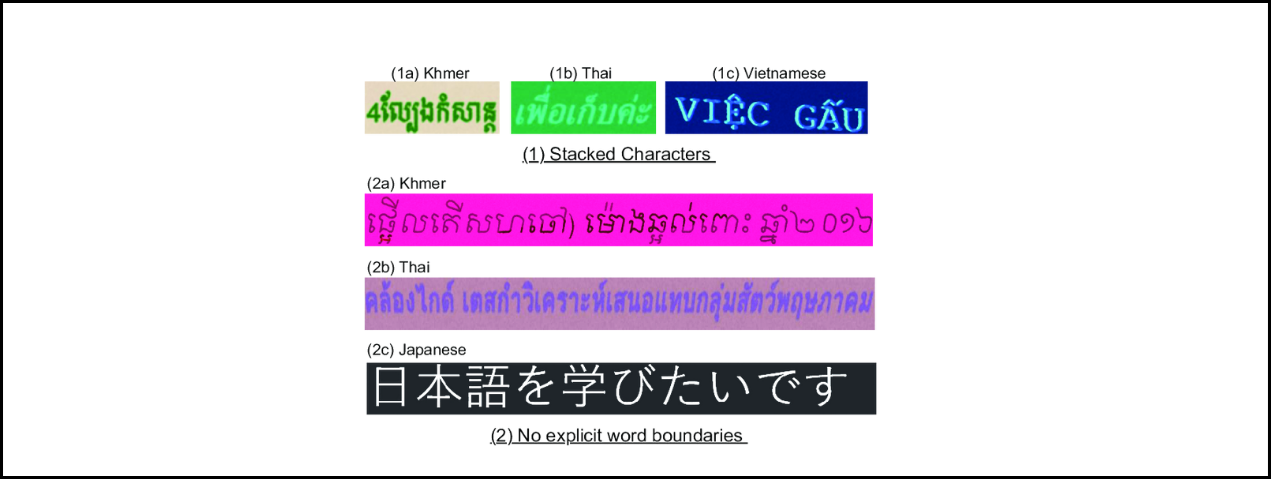
\includegraphics[width=\textwidth]{figures/text_stacking_mixing_language.png}
    \caption{Illustration of Khmer text stacking patterns, 
    showing how characters combine vertically and horizontally 
    to form syllables and words \citep{buoy2023khmerocr}}
    \label{fig:text_stacking}
\end{figure}

That's exactly why we need a better approach. Current OCR tools aren't 
built for the messy reality of Khmer text. They expect perfect conditions
and worked with char-level, word-level only,
that just don't exist in the real world.

\section{Aim and Objectives of the Study}
\label{sec:objectives}

The primary aim of this research is to develop an improved optical character 
recognition (OCR) system specifically designed for MIX-language (Khmer-English) 
addressing the unique challenges of Khmer-English script while achieving high 
accuracy and reliability in real-world applications.

The specific objectives of this study are:

\begin{enumerate}
    \item To create text annotation tool to bounding boxes for create real-dataset for Khmer-English for both text detection and text recognition tasks.
    \item To create a robust training dataset such as varianty of font, real-world environment that addresses the lack of annotated data for Khmer OCR
    \item To develop end-to-end OCR pipelines such as text detection and recognition models that utilizing CRAFT and TrOCR model architectures, particularly focusing on text line based segmentation.
    \item To achieve the state-of-the-art (Accuracy \& CER) and reliability in real-world applications for Khmer-English OCR.
\end{enumerate}

Through achieving these objectives, this research aims to significantly advance the state of Khmer OCR technology and enable more effective digitization of Cambodian textual heritage.

\section{Research Questions}
\label{sec:questions}

This research aims to address the following key questions:

\begin{enumerate}
    \item How can text detection and recognition models be effectively adapted to handle the unique characteristics of Khmer script, particularly the stacking of characters and presence of diacritics?
    
    \item What preprocessing and augmentation techniques are most effective for improving OCR accuracy on Khmer text documents with varying fonts, styles, and quality levels?

    \item What are the minimum dataset requirements and optimal annotation strategies for training robust Khmer OCR models?
    
    \item What is the whole pipeline used to convert document image into digital text on Khmer script with the most Effectiveness?
\end{enumerate}

\section{Rationale of the Study}
\label{sec:rationale}
       This research is motivated by several compelling factors. First, there is an urgent need to digitize and preserve Cambodia's vast textual heritage, including historical documents, educational materials, and cultural artifacts. Without effective OCR technology for Khmer script, this digitization process remains labor-intensive and prone to errors.

Second, the current limitations of OCR systems for Khmer significantly hinder educational and academic initiatives in Cambodia. Many educational institutions struggle to convert physical textbooks and learning materials into digital formats, impacting accessibility and modernization efforts in education.

Third, the unique challenges posed by Khmer script—from character stacking to the absence of word boundaries—present an opportunity to advance the field of OCR technology as a whole. Solutions developed for Khmer may benefit other scripts with similar characteristics.

Finally, improving Khmer OCR technology aligns with broader digital transformation goals in Cambodia, supporting efforts to preserve cultural heritage while enabling more efficient information processing and accessibility in various sectors.

\section{Limitations and Scope}
\label{sec:limitations}

While this research aims to advance Khmer OCR technology significantly, it is important to acknowledge certain limitations and define the scope of the study:

\begin{enumerate}
    \item The research focuses specifically on printed Khmer text and English text and does not address handwritten text recognition, which presents additional challenges requiring separate investigation.
    
    \item The study primarily considers modern Khmer fonts and typography, with limited coverage of historical or decorative text styles.
    
    \item While the system aims to handle various document quality levels, extremely degraded or damaged documents may fall outside the scope of reliable recognition.
    
    \item The study focuses on optical character recognition and does not extend to higher-level natural language processing tasks such as semantic analysis or machine translation.
    
    \item Resource constraints may limit the size and diversity of the training dataset, though efforts will be made to ensure sufficient representation of common use cases.
\end{enumerate}

These limitations help maintain a focused research scope while acknowledging areas that may require future investigation.

\section{Structure of the Thesis}
\label{sec:structure}

This thesis is organized into the following chapters:

\begin{enumerate}
    \item \textbf{Introduction}: Presents the research background, objectives, research questions, rationale, and scope of the study.
    
    \item \textbf{Literature Review}: Reviews existing OCR technologies, challenges in Khmer script recognition, and relevant deep learning approaches.
    
    \item \textbf{Methodology}: Details the proposed approach, including dataset preparation, model architecture, and training procedures.
    
    \item \textbf{Implementation}: Describes the technical implementation, including preprocessing techniques, model modifications, and system integration.
    
    \item \textbf{Results and Analysis}: Presents experimental results, performance analysis, and comparative evaluation with existing solutions.
    
    \item \textbf{Conclusion}: Summarizes key findings, contributions, and suggests directions for future research.
\end{enumerate}
Each chapter builds upon the previous ones to present a comprehensive study of Khmer OCR development.
